%% abtex2-modelo-trabalho-academico.tex, v-1.9.5 laurocesar
%% Copyright 2012-2015 by abnTeX2 group at http://www.abntex.net.br/
%%
%% This work may be distributed and/or modified under the
%% conditions of the LaTeX Project Public License, either version 1.3
%% of this license or (at your option) any later version.
%% The latest version of this license is in
%%   http://www.latex-project.org/lppl.txt
%% and version 1.3 or later is part of all distributions of LaTeX
%% version 2005/12/01 or later.
%%
%% This work has the LPPL maintenance status `maintained'.
%%
%% The Current Maintainer of this work is the abnTeX2 team, led
%% by Lauro César Araujo. Further information are available on
%% http://www.abntex.net.br/
%%
%% This work consists of the files abntex2-modelo-trabalho-academico.tex,
%% abntex2-modelo-include-comandos and abntex2-modelo-references.bib
%%

% ------------------------------------------------------------------------
% ------------------------------------------------------------------------
% abnTeX2: Modelo de Trabalho Academico (tese de doutorado, dissertacao de
% mestrado e trabalhos monograficos em geral) em conformidade com
% ABNT NBR 14724:2011: Informacao e documentacao - Trabalhos academicos -
% Apresentacao
% ------------------------------------------------------------------------
% ------------------------------------------------------------------------

\documentclass[
	% -- opções da classe memoir --
	12pt,				% tamanho da fonte
	%openright,			% capítulos começam em pág ímpar (insere página vazia caso preciso)
	openany, % a chapter can start on any page, then many classes support option openany, e.g.:
	%oneside, % With twoside layout (default for class book) chapters start at odd numbered pages and sometimes LaTeX needs to insert a page to ensure this.
	%twoside,			% para impressão em verso e anverso. Oposto a oneside
	a4paper,			% tamanho do papel.
	% -- opções da classe abntex2 --
	%chapter=TITLE,		% títulos de capítulos convertidos em letras maiúsculas
	%section=TITLE,		% títulos de seções convertidos em letras maiúsculas
	%subsection=TITLE,	% títulos de subseções convertidos em letras maiúsculas
	%subsubsection=TITLE,% títulos de subsubseções convertidos em letras maiúsculas
	% -- opções do pacote babel --
	english,			% idioma adicional para hifenização
	french,				% idioma adicional para hifenização
	spanish,			% idioma adicional para hifenização
	brazil				% o último idioma é o principal do documento
	]{abntex2}

% ---
% Pacotes básicos
% ---
\usepackage{lmodern}			% Usa a fonte Latin Modern
\usepackage[T1]{fontenc}		% Selecao de codigos de fonte.
\usepackage[utf8]{inputenc}		% Codificacao do documento (conversão automática dos acentos)
\usepackage{lastpage}			% Usado pela Ficha catalográfica
\usepackage{indentfirst}		% Indenta o primeiro parágrafo de cada seção.
\usepackage{color}				% Controle das cores
\usepackage{graphicx}			% Inclusão de gráficos
\usepackage{microtype} 			% para melhorias de justificação
\usepackage{booktabs}
\usepackage{graphicx}
\usepackage[table,xcdraw]{xcolor}
\usepackage{float}
\usepackage{listings}
\usepackage{ragged2e}


% --- https://www.overleaf.com/learn/latex/Code_listing



\usepackage{xcolor}
\renewcommand\lstlistingname{Lista de código}
\renewcommand\lstlistlistingname{Lista de trechos de código}

% https://tex.stackexchange.com/questions/111580/removing-an-unwanted-page-between-two-chapters
\let\cleardoublepage\clearpage % Unwanted one-page gap between two chapters can be eliminated using the syntax




\definecolor{codegreen}{rgb}{0,0.6,0}
\definecolor{codegray}{rgb}{0.5,0.5,0.5}
\definecolor{codepurple}{rgb}{0.58,0,0.82}
\definecolor{backcolour}{rgb}{0.95,0.95,0.92}

\lstdefinestyle{mystyle}{
    backgroundcolor=\color{backcolour},
    commentstyle=\color{codegreen},
    keywordstyle=\color{magenta},
    numberstyle=\tiny\color{codegray},
    stringstyle=\color{codepurple},
    basicstyle=\ttfamily\footnotesize,
    breakatwhitespace=false,
    breaklines=true,
    captionpos=b,
    keepspaces=true,
    numbers=left,
    numbersep=5pt,
    showspaces=false,
    showstringspaces=false,
    showtabs=false,
    tabsize=2
}

\lstset{style=mystyle}





% ---
% Pacotes adicionais, usados apenas no âmbito do Modelo Canônico do abnteX2
% ---
\usepackage{lipsum}				% para geração de dummy text
% ---

% ---
% Pacotes de citações
% ---
\usepackage[brazilian,hyperpageref]{backref}	 % Paginas com as citações na bibl
\usepackage[alf]{abntex2cite}	% Citações padrão ABNT

% ---
% First pip install pygments

% CONFIGURAÇÕES DE PACOTES
% ---

% ---
% Configurações do pacote backref
% Usado sem a opção hyperpageref de backref
\renewcommand{\backrefpagesname}{Citado na(s) página(s):~}
% Texto padrão antes do número das páginas
\renewcommand{\backref}{}
% Define os textos da citação
\renewcommand*{\backrefalt}[4]{
	\ifcase #1 %
		Nenhuma citação no texto.%
	\or
		Citado na página #2.%
	\else
		Citado #1 vezes nas páginas #2.%
	\fi}%
% ---

% ---
% Informações de dados para CAPA e FOLHA DE ROSTO
% ---
\titulo{Inteligência artificial e Chatbots: \\um estudo prático}
\autor{Daniel Terra Gomes, Andre do Valle Medeiros}
\local{Campos dos Goytacazes, RJ}
\data{\today, v1.0.0}
%\orientador{Manuel Antonio Molina Palma}
%\coorientador{Equipe \abnTeX}
\instituicao{%
Universidade Estadual do Norte Fluminense Darcy Ribeiro
  \par
  Ciência da Computação
  \par
  INF01205 - IA 2022}
\tipotrabalho{Projeto de Pesquisa}
% O preambulo deve conter o tipo do trabalho, o objetivo,
% o nome da instituição e a área de concentração
\preambulo{Relatório Atividade 1 apresentado ao Curso de Ciência da Computação da
Universidade Estadual do Norte Fluminense
Darcy Ribeiro, como requisito avaliativo da
disciplina.}
% ---


% ---
% Configurações de aparência do PDF final

% alterando o aspecto da cor azul
\definecolor{blue}{RGB}{41,5,195}

% informações do PDF
\makeatletter
\hypersetup{
     	%pagebackref=true,
		pdftitle={\@title},
		pdfauthor={\@author},
    	pdfsubject={\imprimirpreambulo},
	    pdfcreator={LaTeX with abnTeX2},
		pdfkeywords={abnt}{latex}{abntex}{abntex2}{trabalho acadêmico},
		colorlinks=true,       		% false: boxed links; true: colored links
    	linkcolor=blue,          	% color of internal links
    	citecolor=blue,        		% color of links to bibliography
    	filecolor=magenta,      		% color of file links
		urlcolor=blue,
		bookmarksdepth=4
}
\makeatother
% ---

% ---
% Espaçamentos entre linhas e parágrafos
% ---

% O tamanho do parágrafo é dado por:
\setlength{\parindent}{1.3cm}

% Controle do espaçamento entre um parágrafo e outro:
\setlength{\parskip}{0.2cm}  % tente também \onelineskip

% ---
% compila o indice
% ---
\makeindex
% ---

% ----
% Início do documento
% ----
\begin{document}

% Seleciona o idioma do documento (conforme pacotes do babel)
%\selectlanguage{english}
\selectlanguage{brazil}

% Retira espaço extra obsoleto entre as frases.
\frenchspacing

% ----------------------------------------------------------
% ELEMENTOS PRÉ-TEXTUAIS
% ----------------------------------------------------------
% \pretextual

% ---
% Capa
% ---
\imprimircapa
% ---

% ---
% Folha de rosto
% (o * indica que haverá a ficha bibliográfica)
% ---
\imprimirfolhaderosto*
% ---

% ---
% Inserir a ficha bibliografica
% ---

% Isto é um exemplo de Ficha Catalográfica, ou ``Dados internacionais de
% catalogação-na-publicação''. Você pode utilizar este modelo como referência.
% Porém, provavelmente a biblioteca da sua universidade lhe fornecerá um PDF
% com a ficha catalográfica definitiva após a defesa do trabalho. Quando estiver
% com o documento, salve-o como PDF no diretório do seu projeto e substitua todo
% o conteúdo de implementação deste arquivo pelo comando abaixo:
%
% \begin{fichacatalografica}
%     \includepdf{fig_ficha_catalografica.pdf}
% \end{fichacatalografica}

%\begin{fichacatalografica}
%	\sffamily
%	\vspace*{\fill}					% Posição vertical
%	\begin{center}					% Minipage Centralizado
%	\fbox{\begin{minipage}[c][8cm]{13.5cm}		% Largura
%	\small
%	\imprimirautor
%	%Sobrenome, Nome do autor
%
%	\hspace{0.5cm} \imprimirtitulo  / \imprimirautor. --
%	\imprimirlocal, \imprimirdata-
%
%	\hspace{0.5cm} \pageref{LastPage} p. : il. \\ % (algumas color.) ; 30 cm.\\
%
%	\hspace{0.5cm} \imprimirorientadorRotulo~\imprimirorientador\\
%
%	\hspace{0.5cm}
%	\parbox[t]{\textwidth}{\imprimirtipotrabalho~--~\imprimirinstituicao,
%	\imprimirdata.}\\
%
%	\hspace{0.5cm}
%		1. Veículos autônomos.
%		2. Inteligência Artificial.
%		3. Machine Learning.
%		4. Condução Autônoma.
%		I. Manuel Antonio Molina Palma.
%		II. Universidade Estadual do Norte Fluminense Darcy Ribeiro.
%		III. Faculdade de Ciência da Computação.
%		IV. Veículos autônomos e inteligência artificial:
% um estudo sobre a implementação no brasil.
%	\end{minipage}}
%	\end{center}
%\end{fichacatalografica}
% ---

% ---
% Inserir errata
% ---

% Inserir folha de aprovação
% ---

% Isto é um exemplo de Folha de aprovação, elemento obrigatório da NBR
% 14724/2011 (seção 4.2.1.3). Você pode utilizar este modelo até a aprovação
% do trabalho. Após isso, substitua todo o conteúdo deste arquivo por uma
% imagem da página assinada pela banca com o comando abaixo:
%
% \includepdf{folhadeaprovacao_final.pdf}
%
\begin{folhadeaprovacao}

	\begin{center}
		{\ABNTEXchapterfont\large\imprimirautor}

		\vspace*{\fill}\vspace*{\fill}
		\begin{center}
			\ABNTEXchapterfont\bfseries\Large\imprimirtitulo
		\end{center}
		\vspace*{\fill}

		\hspace{.45\textwidth}
		\begin{minipage}{.5\textwidth}
			\imprimirpreambulo
		\end{minipage}%
		\vspace*{\fill}
	\end{center}
	% \begin{center}
	%	\imprimirlocal, \today
	%\end{center}
	%%%%%%%%%%%%\assinatura{\textbf{\imprimirorientador} \\ Orientador}

	%\assinatura{\textbf{Professor} \\ Convidado 1}
	% \assinatura{\textbf{Professor} \\ Convidado 2}
	%\assinatura{\textbf{Professor} \\ Convidado 3}
	%\assinatura{\textbf{Professor} \\ Convidado 4}

	\begin{center}
		\vspace*{0.5cm}
		{\large\imprimirlocal}
		\par
		{\large\imprimirdata}
		\vspace*{1cm}
	\end{center}

\end{folhadeaprovacao}
% ---

% ---
% Dedicatória
% ---
\begin{dedicatoria}
	\vspace*{\fill}
	\centering
	\noindent
	\textit{ Este trabalho é dedicado às crianças adultas que,\\
		quando pequenas, sonharam em se tornar cientistas.} \vspace*{\fill}
\end{dedicatoria}
% ---

% ---
% Agradecimentos
% ---
%%%%\begin{agradecimentos}
%%%%Agradeço aos meus pais que se dedicaram para que eu pudesse estar cursando esta graduação, assim podendo completar mais uma etapa da minha vida.
%%%%Sem o apoio, conselhos, carinho e amor, nada disso seria possível. Sou eternamente grato por tudo que vocês fazem e sempre fizeram para que minha vida fosse especial.
%%%%
%%%%Agradeço ao professor Dr. Manuel Antonio Molina Palma pela dedicação e paciência durante o lecionamento desta disciplina, e obrigado pela ajuda e por estar disponível nos momentos de necessidade.
%%%%
%%%%Por último, mas não menos importante, agradeço a toda minha família e amigos que estiveram comigo em todos os momentos da minha vida.
%%%%
%%%%
%%%%\end{agradecimentos}
% ---

% ---
% Epígrafe
% ---
\begin{epigrafe}
	\vspace*{\fill}
	\begin{flushright}
		\textit{``Behind me lies a farm. \\
			I wonder if there is bread above the hearth \\
			and if I will ever return. \\
			(Pantheon, League of Legends)}
	\end{flushright}
\end{epigrafe}
% ---

% ---
% RESUMOS
% ---

% resumo em português
% resumo em inglês
\begin{resumo}[Abstract]
	\begin{otherlanguage*}{english}
		This article provides an introduction to AI and Chatbots. Communicating with customers through chat interfaces has, in recent years, become an increasingly popular means of providing real-time customer service in many e-commerce environments. Today, human chat service agents are often replaced by conversational software agents or chatbots, which are systems designed to communicate with human users using Machine Learning (ML) techniques such as Natural Language Processing (NLP), usually based on artificial intelligence (AI). Advances in these areas, particularly in Deep Learning, coupled with the availability of vast computational power and large amounts of data, have led to a new generation of dialog systems and conversational interfaces. Enabling even greater advances in AI. In the practical project developed in this article, we developed a simple Chatbot using 2 neural layers to process messages sent by a user. In this way, it was possible to achieve the desired objective of responding to users with responses from our training base.
		\vspace{\onelineskip}

		\noindent
		\textbf{Keywords}: Chatbots. Artificial Intelligence. Machine Learning.
	\end{otherlanguage*}
\end{resumo}
\setlength{\absparsep}{18pt} % ajusta o espaçamento dos parágrafos do resumo
\begin{resumo}[Resumo]
	\begin{otherlanguage*}{portuguese}
		Este artigo fornece uma introdução à IA e Chatbots. A comunicação com os clientes por meio de interfaces de bate-papo, nos últimos anos, tornou-se um meio cada vez mais popular de fornecer atendimento ao cliente em tempo real em muitos ambientes de comércio eletrônico. Hoje, os agentes de serviço de bate-papo humano são frequentemente substituídos por agentes de software de conversação ou chatbots, que são sistemas projetados para se comunicar com usuários humanos usando técnicas de Machine Learning (ML) como o Processamento de Linguagem Natural (PLN), geralmente baseada em inteligência artificial (IA).
		Avanços nessas áreas, particularmente em Deep Learning, juntamente com a disponibilidade de grande poder computacional e grandes quantidades de dados, levaram a uma nova geração de sistemas de diálogo e interfaces de conversação. Possibilitando avanços ainda maiores em IA.
		No projeto prático desenvolvido neste artigo elaboramos um Chatbot simples fazendo uso de 2 camadas neurais para o processamento de mensagens enviadas por um usuários.
		Desse modo, foi possível  alcançar o objetivo desejado de responder os usuários com respostas da nossa base de treino.
		\vspace{\onelineskip}

		\noindent
		\textbf{Palavras-chave}: Chatbots. Inteligência Artificial. Machine Learning.
	\end{otherlanguage*}
\end{resumo}


%%%%%%%%%%%
% ---
% inserir lista de ilustrações
% ---
\pdfbookmark[0]{\listfigurename}{lof}
\listoffigures*
\cleardoublepage
% ---

% ---
% inserir lista de tabelas
% ---
%\pdfbookmark[0]{\listtablename}{lot}
%\listoftables*
%\cleardoublepage

\pdfbookmark[0]{\lstlistingname}{lop}%
\lstlistoflistings


% ---

% ---
% inserir lista de abreviaturas e siglas
% ---
\begin{siglas}
	\item[NLP] Natural language processing
	\item[ML] Machine Learning
	\item[IA] Inteligência Artificial
\end{siglas}
% ---

% ---
% inserir lista de símbolos
% ---


% ---
% inserir o sumario
% ---
\pdfbookmark[0]{\contentsname}{toc}
\tableofcontents*
\cleardoublepage
% ---



% ----------------------------------------------------------
% ELEMENTOS TEXTUAIS
% ----------------------------------------------------------
\textual

% ----------------------------------------------------------
% Introdução (exemplo de capítulo sem numeração, mas presente no Sumário)
% ----------------------------------------------------------
\chapter*[Projeto de Pesquisa]{Introdução}
\addcontentsline{toc}{chapter}{Introdução}
% ----------------------------------------------------------

Nosso projeto propõe a implementação de um Chatbot é um software ou programa de computador que simula conversas humanas por meio de interações de texto ou voz, permitindo que os humanos interajam com dispositivos digitais como se estivessem se comunicando com uma pessoa real. Os chatbots podem ser tão simples quanto programas rudimentares que respondem a uma consulta simples com uma resposta de linha única ou tão sofisticados quanto assistentes digitais que aprendem e evoluem para fornecer níveis crescentes de personalização à medida que coletam e processam informações.

Você provavelmente já interagiu com um chatbot, sabendo ou não. Por exemplo, você está em seu computador pesquisando um produto e uma janela aparece na tela perguntando se você precisa de ajuda. Ou talvez você esteja a caminho de um show e use seu smartphone para solicitar uma carona via chat. Ou você pode ter usado comandos de voz para pedir um café no café do bairro e receber uma resposta informando quando seu pedido estará pronto e quanto custará. \footnote{\url{https://www.oracle.com/chatbots/what-is-a-chatbot/}}.

Esses sistemas de Chats podem ser divididos entre dos tipos; orientados a objetivo (Chatbots) que seriam chats que ajudam o usuários a atingir um certo objetivo e com um campo de conhecimento restrito e, também há os Chit Chat cujo trabalham com perguntas abertas, respostas mais naturais e campo de conhecimento aberto de modo a ajudar a encontrar uma informação (QA System) \footnote{\url{https://youtu.be/Mu1N-akGL78}}.

Um aspecto crítico da implementação do chatbot é selecionar o mecanismo correto de processamento de linguagem natural (NLP) \footnote{\url{https://www.techtarget.com/searchcustomerexperience/definition/chatbot/}}.
Esse mecanismo conhecido como NLP O refere-se ao ramo da ciência da computação – e mais especificamente, o ramo da inteligência artificial ou IA – preocupado em dar aos computadores a capacidade de entender texto e palavras faladas da mesma maneira que os seres humanos.
A NLP combina linguística computacional – modelagem baseada em regras da linguagem humana – com modelos estatísticos, de aprendizado de máquina e aprendizado profundo. Juntas, essas tecnologias permitem que os computadores processem a linguagem humana na forma de texto ou dados de voz e 'compreendam' seu significado completo, completo com a intenção e o sentimento do falante ou escritor \footnote{\url{https://www.ibm.com/cloud/learn/natural-language-processing}}.

Sendo assim, propomos realizar uma implementação de um Chatbot Simples (jump to define) capaz de auxiliar um usuário durante uma compra em um Website. Durante o desenvolvimento deste projeto estaremos realizando uma pesquisa exploratória a fim de entender o funcionamento de um Software que aplica NLP.
Por consequência, ao final deste projeto teremos implementado e apresentado o nosso sistema de Chatbot, e compreendido as tecnologias para o seu funcionamento. Assim alcançando uma aprendizagem eficaz, autodidata, e exploratória.



% PARTE
% ----------------------------------------------------------
%\part{Preparação da pesquisa}
% ----------------------------------------------------------

% ---
% Capitulo com exemplos de comandos inseridos de arquivo externo
% ---
%\include{abntex2-modelo-include-comandos}
% ----------------------------------------------------------


\chapter[Fundamentação Teórica]{Fundamentação Teórica}\label{Fundamentacao}
\begin{enumerate}
   \item  Como contribuição teórica inicial para o nosso projeto, temos o material do canal no Youtube 'Python Engineer' a playlist de vídeo aulas,  'Chat Bot With PyTorch - NLP Beginner Tutorial' \footnote{\url{https://www.youtube.com/playlist?list=PLqnslRFeH2UrFW4AUgn-eY37qOAWQpJyg}}. A partir desse conteúdo poderemos dar início aos nossos desenvolvimentos e pesquisas. No tutorial, é desenvolvido um chatbot simples usando PyTorch e Deep Learning. Também fornecendo uma introdução a algumas técnicas básicas de Processamento de Linguagem Natural (PLN).

   \item Seguiremos, também, os conteúdos já aprendidos nas aulas de  'Inteligência Artifical 2022/2 - UENF' para nos auxiliar na formulação teórica do nosso projeto.

   \item  Salientamos que com o decorrer do projeto nossas referências de materiais, para esse projeto, tenderá a aumentar devido a novas descobertas.
\end{enumerate}







\chapter[Metodologia]{Metodologia}

Baseado no “Project-based learning” \cite{krajcik2006project}. Seguiremos os estudos através de um projeto que aborda problemas do mundo real, cujo muitos não tem resposta única. Ao longo desse projeto será possível fazer novas perguntas e encontrar suas possíveis respostas por meio de uma investigação sustentada.

\justifying
\vspace {1mm}

Este Plano de Pesquisa também utilizará as seguintes metodologias:
\begin{itemize}
   \item \textit{Pesquisa Exploratória; visando promover o enriquecimento do conhecimento sobre os diferentes assuntos relacionados a IA, ML, e Chatbots:
         }
         \begin{itemize}
            \item \textit{Levantamento Bibliográfico;}
            \item \textit{Levantamento documental;}
            \item \textit{Minicursos e Vídeo aulas;}
            \item \textit{Obtenção de experiências.}
         \end{itemize}
\end{itemize}

\chapter[Construindo um Chatbot com Pytorch]{Construindo um Chatbot com Pytorch}

Já pensou em como Alexa, Siri ou assistente de voz do Google funcionavam? Neste capítulo daremos início à construção de um chatbot para interação com usuários de uma loja virtual.

Antes de continuar, abaixo encontra-se a lista de requisitos para o nosso projeto:
\justifying
\begin{itemize}
   \item \textit{Python 3}
         \begin{itemize}
            \item \textit{Define: Python} é uma linguagem de programação interpretada, orientada a objetos e de alto nível com semântica dinâmica. Suas estruturas de dados embutidas de alto nível, combinadas com tipagem dinâmica e vinculação dinâmica, o tornam muito atraente para o Desenvolvimento Rápido de Aplicativos e para uso como uma linguagem de script ou cola para conectar componentes existentes \footnote{\url{https://www.python.org/doc/essays/blurb/}}.
         \end{itemize}

   \item \textit{Dictionaries e Lists}
         \begin{itemize}
            \item \textit{Define: Listas} são tipos de dados mutáveis em Python. Lists é um tipo de dados de índice baseado em 0, o que significa que o índice do primeiro elemento começa em 0. As listas são usadas para armazenar vários itens em uma única variável. As listas são um dos 4 tipos de dados do Python, ou seja, Listas, Dicionário, Tupla e Conjunto \footnote{\url{https://www.analyticsvidhya.com/blog/2021/06/working-with-lists-dictionaries-in-python/}}.
            \item \textit{Define: Dicionários} Dicionários são a implementação do Python de uma estrutura de dados que é mais conhecida como uma matriz associativa. Um dicionário consiste em uma coleção de pares chave-valor. Cada par de chave-valor mapeia a chave para seu valor associado\footnote{\url{https://realpython.com/python-dicts}}.
         \end{itemize}

   \item \textit{NumPy}
         \begin{itemize}
            \item \textit{Define: NumPy} é o pacote fundamental para computação científica em Python. É uma biblioteca Python que fornece um objeto array multidimensional, vários objetos derivados (como arrays e matrizes mascarados) e uma variedade de rotinas para operações rápidas em arrays, incluindo matemática, lógica, manipulação de formas, classificação, seleção, E/S , Fourier discreto transforma álgebra linear básica, operações estatísticas básicas, simulação aleatória e muito mais\footnote{\url{https://numpy.org/doc/stable/user/whatisnumpy.html}}.
         \end{itemize}

   \item \textit{Pandas}
         \begin{itemize}
            \item \textit{Define: Pandas} é um pacote Python de código aberto que é mais amplamente usado para ciência de dados/análise de dados e tarefas de aprendizado de máquina. Ele é construído em cima de outro pacote chamado Numpy, que fornece suporte para arrays multidimensionais\footnote{\url{https://www.activestate.com/resources/quick-reads/what-is-pandas-in-python-everything-you-need-to-know/}}.
         \end{itemize}

   \item \textit{Pytorch}
         \begin{itemize}
            \item \textit{Define: PyTorch} é uma biblioteca de aprendizado de máquina para Python usada principalmente para processamento de linguagem natural. O software de código aberto foi desenvolvido pelas equipes de inteligência artificial do Facebook Inc. em 2016. O PyTorch oferece dois recursos significativos, incluindo computação de tensor, bem como redes neurais profundas funcionais\footnote{\url{https://deepai.org/machine-learning-glossary-and-terms/pytorch}}.
         \end{itemize}

   \item \textit{Natural Language Processing (Bag of Words)}
         \begin{itemize}
            \item \textit{Define: NLP ou PLN }O processamento de linguagem natural usa aprendizado de máquina para revelar a estrutura e o significado do texto. Com aplicativos de processamento de linguagem natural, as organizações podem analisar texto e extrair informações sobre pessoas, lugares e eventos para entender melhor o sentimento da mídia social e as conversas com os clientes \footnote{\url{https://cloud.google.com/learn/what-is-natural-language-processing}}.
         \end{itemize}


\end{itemize}

\section[Importando Bibliotecas Relevantes]{Importando Bibliotecas Relevantes}
\begin{lstlisting}[language=Python, caption=Python Bibliotecas]

   import numpy as np
   import random
   import json
   import nltk
   import torch
   import torch.nn as nn
   from torch.utils.data import Dataset, DataLoader
\end{lstlisting}


\section[Criando funções personalizadas]{Criando funções personalizadas}
Criaremos funções personalizadas para que seja fácil implementá-las posteriormente.
\justifying
\begin{lstlisting}[language=Python, caption=Python Funções personalizadas]
def tokenize(sentence):
    return nltk.word_tokenize(sentence)

def stem(word):
    return stemmer.stem(word.lower())

\end{lstlisting}
Nltk ou kit de ferramentas de linguagem natural é uma biblioteca realmente útil que contém classes importantes que serão úteis em qualquer uma de suas tarefas de PNL.
\justifying
\section[Stemming]{Stemming}


Se tivermos as seguintes palavras como Andei, Ande, Andarei, Andamento, Andando, Andante, podem parecer palavras diferentes, mas geralmente têm o mesmo significado e também a mesma forma base; "and".
O processo de stemização (do inglês, stemming) consiste em reduzir uma palavra ao seu radical. A palavra “meninas” se reduziria a “menin”, assim como “meninos” e “menininhos”. As palavras “gato”, “gata”, “gatos” e “gatas” reduziriam-se para “gat” \footnote{\url{https://www.computersciencemaster.com.br/como-reduzir-uma-palavra-ao-seu-radical-em-python-stemming/}}.
Então, para que nosso modelo entenda todas as formas diferentes das mesmas palavras, precisamos treinar nosso modelo com essa forma. Isso é chamado de Stemming. Existem diferentes métodos que podemos usar para derivação. Aqui usaremos o modelo Porter Stemmer da nossa biblioteca NLTK.
\justifying
\begin{lstlisting}[language=Python, caption=Python Stemming]
from nltk.stem.porter import PorterStemmer
stemmer = PorterStemmer()
\end{lstlisting}

\section[Bag of Words]{Bag of Words}
Vamos dividir cada palavra em frases e adicioná-la a um array. Nós estaremos usando um saco de palavras. Que inicialmente será uma lista de zeros com um tamanho igual ao comprimento do array all-words. Se tivermos um array de ` frases = ["ola", "como", "voce", "esta"]` e um array de total ` words = ["oi", "olá", "eu", "você, "tchau", "obrigado", "legal"]` então seu conjunto de palavras será `bog = [ 0 , 1 , 0 , 1 , 0 , 0 , 0]`. Faremos um loop sobre cada palavra no array all-words e o array bog correspondente a cada palavra. Se uma palavra da frase for encontrada no array all words, 1 será substituído naquele índice/posição no array bag.
\justifying


\begin{figure}[H]
   \begin{center}
      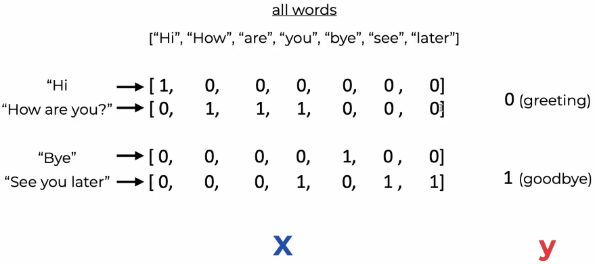
\includegraphics[width=15cm]{img/bagofwords.png}
      \caption{Bag of Words} \label{BagofWords}
      \medskip
      \small
      Usa Bag of Words para separar uma frase em várias palavras. Imagem retirada da Fundamentação Teórica \ref{Fundamentacao}.
   \end{center}
\end{figure}


\begin{lstlisting}[language=Python, caption=Python Bag of Words]
def bag_of_words(tokenized_sentence, words):
    """
    return bag of words array:
    1 para cada palavra conhecida que existe na frase,
    0 caso contrario.


    Exem,plo:


    sentence = ["ola", "como", "esta", "voce"]
    words = ["oi", "ola", "eu", "voce", "tchau",
     "obrigado", "legal"]
    bag   = [  0 ,    1 ,    0 ,   1 ,    0 ,    0 ,      0]
    """
    # stem cada palavra
    sentence_words = [stem(word) for word in tokenized_sentence]
    # initialize bag com 0 para cada palavra
    bag = np.zeros(len(words), dtype=np.float32)
    for idx, w in enumerate(words):
        if w in sentence_words:
            bag[idx] = 1

    return bag

\end{lstlisting}

Durante o processo, também usaremos \textbf{nltkwordtokenize()} que converterá uma única string de sentença em uma lista de palavras. Por exemplo, se você passar \textbf{"Ola, como voce esta?"}, ele retornará \textbf{"ola", "como", "voce", "esta"}.
\textbf{Observação:} Passaremos palavras em minúsculas para o \textbf{Stemmer} para que palavras como Bom e bom (em maiúsculas) não sejam rotuladas como palavras diferentes.

\section[Carregando os dados e Data Cleaning]{Carregando os dados e Data Cleaning}
Usaremos um conjunto de dados chamado  \textbf{intents.json} que tem a estrutura mostrada no campo abaixo. Estaremos limpando esses dados de acordo com as nossas necessidades usando as funções que criamos anteriormente.

\begin{lstlisting}[language=python, caption=Data intents.json]
{
  "intents": [
    {
      "tag": "saudacao",
      "patterns": [
        "Oi",
        "Ei",
        "Como voce esta",
        "Tem alguem ai?",
        "Ola",
        "Bom dia"
      ],
      "responses": [
        "Ei :-)",
        "Ola, obrigado pela visita",
        "Ola, o que posso fazer por voce?",
        "Ola, como posso ajudar?"
      ]
   }
  ]
}


\end{lstlisting}
Agora vamos simplesmente carregar o arquivo json usando a função \textbf{jsonload}.

\begin{lstlisting}[language=Python, caption=Python Carregando dados]
with open('intents.json', 'r') as f:
    intents = json.load(f)
\end{lstlisting}

Para obter as informações corretas, iremos descompactá-las com o seguinte código:

\begin{lstlisting}[language=Python, caption=Python Loop nos dados]
all_words = []
tags = []
xy = []
# loop atraves de cada frase no nosso intents patterns
for intent in intents['intents']:
    tag = intent['tag']
    # adicionar a tag list
    tags.append(tag)
    for pattern in intent['patterns']:
        # tokenize cada palavra na frase
        w = tokenize(pattern)
        # adicionar a nossa lista de palavras
        all_words.extend(w)
        # adicionar ao par xy
        xy.append((w, tag))

\end{lstlisting}
Isso separará todas as tags e palavras em suas listas.

\section[Limpeza e preparação dos dados]{Limpeza e preparação dos dados}


Estaremos usando nossas funções personalizadas e limpando os dados implementando as funções que criamos em nossas células anteriores.

\begin{lstlisting}[language=Python, caption=Data Cleaning]

# stem e lower cada palavra
ignore_words = ['?', '.', '!']
all_words = [stem(w) for w in all_words if w not in ignore_words]
# remover duplicados e sort
all_words = sorted(set(all_words))
tags = sorted(set(tags))

print(len(xy), "patterns") # padroes
print(len(tags), "tags:", tags) # tags
print(len(all_words), "unique stemmed words:", all_words) # palavras derivadas unicas

\end{lstlisting}

Criando dados de treinamento: transformaremos os dados em um formato que nosso modelo PyTorch possa entender facilmente

\begin{lstlisting}[language=Python, caption=Training Data]

# criar dados de treinamento
X_train = []
y_train = []
for (pattern_sentence, tag) in xy:
    # X: bag de palavras para cada pattern_sentence
    bag = bag_of_words(pattern_sentence, all_words)
    X_train.append(bag)
    # y: PyTorch CrossEntropyLoss precisa apenas class labels, nao one-hot
    label = tags.index(tag)
    y_train.append(label)

X_train = np.array(X_train)
y_train = np.array(y_train)

\end{lstlisting}

\section[Modelo PyTorch]{Modelo PyTorch}

Aqui estaremos fazendo uma classe para implementar nossa rede neural personalizada. Será uma Rede neural feed-forward que terá 3 Camadas Lineares e usaremos a função de ativação “ReLU”. Nota: Usamos a função super() para herdar as propriedades de sua classe pai. Este é um conceito de Programação Orientada a Objetos (OOP).

\begin{itemize}
   \item \textit{Define: ReLU} é uma função de ativação não linear que é usada em redes neurais multicamadas ou redes neurais profundas. Esta função pode ser representada como:

         \begin{figure}[H]
            \begin{center}
               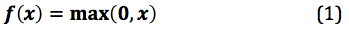
\includegraphics[width=10cm]{img/relu.jpg}
               \caption{ReLu} \label{ReLu}
               \medskip
               \small
               onde x = um valor de entrada.
            \end{center}
         \end{figure}

         De acordo com a equação 1, a saída de ReLu é o valor máximo entre zero e o valor de entrada. A saída é igual a zero quando o valor de entrada é negativo e o valor de entrada quando a entrada é positiva. Assim, podemos reescrever a equação 1 da seguinte forma:

         \begin{figure}[H]
            \begin{center}
               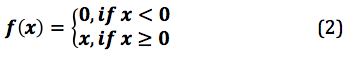
\includegraphics[width=10cm]{img/relu2.jpg}
               \caption{ReLu} \label{ReLu2}
               \medskip
               \small
               onde x = um valor de entrada.
            \end{center}
         \end{figure}


         Exemplos de ReLu: Dadas diferentes entradas, a função gera diferentes saídas. Por exemplo, quando x é igual a -5, a saída de f(-5) é 0. Por outro lado, a saída de f(0) é 0 porque a entrada é maior ou igual a 0. Além disso, o resultado de f (5) é 5 porque a entrada é maior que zero \footnote{\url{https://deepai.org/machine-learning-glossary-and-terms/relu/}}.
\end{itemize}

\subsection[Feed Forward Neural Network]{Feed Forward Neural Network}

\textit{Define: Feed Forward Neural Network} Uma Rede Neural Feed Forward é uma rede neural artificial na qual as conexões entre os nós não formam um ciclo. O oposto de uma rede neural feed-forward é uma rede neural recorrente, na qual certos caminhos são ciclados. O modelo feed-forward é a forma mais simples de uma rede neural, pois a informação é processada apenas em uma direção. Embora os dados possam passar por vários nós ocultos, eles sempre se movem em uma direção e nunca para trás \footnote{\url{https://deepai.org/machine-learning-glossary-and-terms/feed-forward-neural-network}}.


\begin{figure}[H]
   \begin{center}
      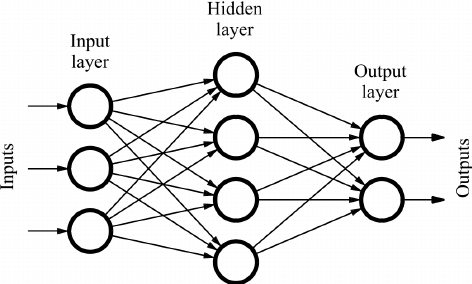
\includegraphics[width=10cm]{img/ffnn.png}
      \caption{Feed Forward Neural Network} \label{ffnn}
      \medskip
      \small
      Exemplo de uma rede neural feed-forward.
   \end{center}
\end{figure}

Desse modo, uma representação válida para o nosso projeto seria a FFNN abaixo:
\begin{figure}[H]
   \begin{center}
      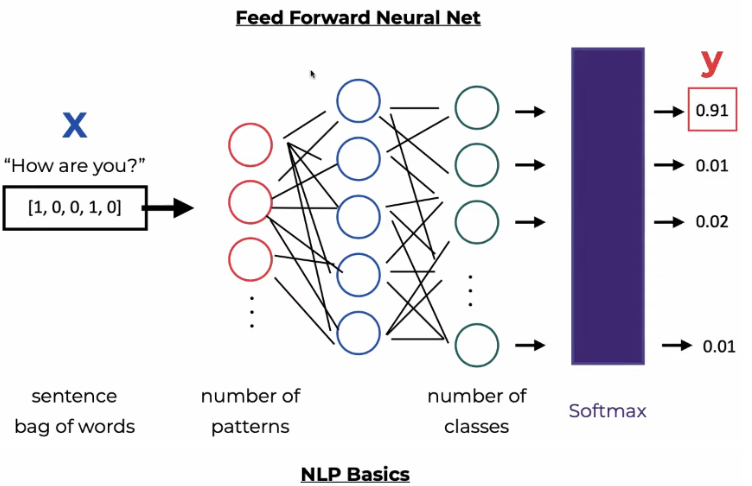
\includegraphics[width=10cm]{img/ffnn2.png}
      \caption{Feed Forward Neural Network} \label{ffnn2}
      \medskip
      \small
      Exemplo de uma rede neural feed-forward para o nosso projeto. Imagem retirada da Fundamentação Teórica \ref{Fundamentacao}.
   \end{center}
\end{figure}

\subsection[Função de ativação]{Função de ativação}

\textit{Define: Função de ativação} Uma função de ativação é uma função usada em redes neurais artificiais que produz um valor pequeno para entradas pequenas e um valor maior se suas entradas excederem um limite. Se as entradas forem grandes o suficiente, a função de ativação "dispara", caso contrário não faz nada. Em outras palavras, uma função de ativação é como um portão que verifica se um valor de entrada é maior que um número crítico.

As funções de ativação são úteis porque adicionam não linearidades às redes neurais, permitindo que as redes neurais aprendam operações poderosas. Se as funções de ativação fossem removidas de uma rede neural feedforward, toda a rede poderia ser refatorada para uma simples operação linear ou transformação de matriz em sua entrada e não seria mais capaz de realizar tarefas complexas, como reconhecimento de imagem \footnote{\url{https://towardsdatascience.com/activation-functions-neural-networks-1cbd9f8d91d6}}.

\subsubsection[Função ReLU]{Função ReLU}
Atualmente, existem várias funções de ativação amplamente usadas no aprendizado profundo. Uma das mais simples é a ReLU (Rectified Linear Unit) Activation Function, ou função ReLU, que é uma função linear por partes que produz zero se sua entrada for negativa, e diretamente a saída caso contrário.
Como mencionado, O ReLU é a função de ativação mais usada no mundo atualmente. Já que é usado em quase todas as redes neurais convolucionais ou deep learning.

\begin{figure}[H]
   \begin{center}
      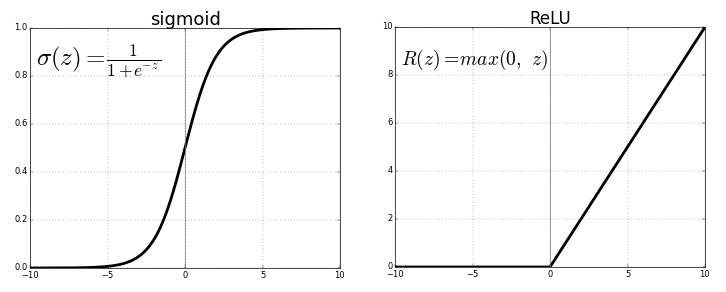
\includegraphics[width=10cm]{img/relu.png}
      \caption{ReLU v/s Logistic Sigmoid} \label{relu}
   \end{center}
\end{figure}
Como você pode identificar, o ReLU está meio retificado (de baixo). f(z) é zero quando z é menor que zero e f(z) é igual a z quando z é maior ou igual a zero.

Range: [ 0 ao infinito)

A função e sua derivada são monotônicas.

Mas o problema é que todos os valores negativos se tornam zero imediatamente, o que diminui a capacidade do modelo de ajustar ou treinar a partir dos dados corretamente. Isso significa que qualquer entrada negativa dada à função de ativação ReLU transforma o valor em zero imediatamente no gráfico, o que, por sua vez, afeta o gráfico resultante por não mapear os valores negativos adequadamente\footnote{\url{https://towardsdatascience.com/activation-functions-neural-networks-1cbd9f8d91d6}}.

\subsubsection[Derivada da Função ReLU]{Derivada da Função ReLU}

Em redes neurais, uma função de ativação agora comumente usada é a unidade linear retificada, ou como comumente abreviada, ReLU. O ReLU é definido como,

\begin{figure}[H]
   \begin{center}
      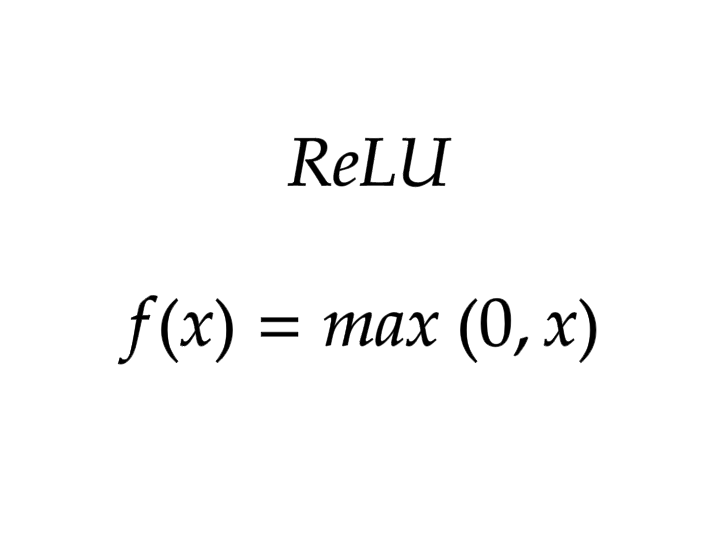
\includegraphics[width=10cm]{img/relu2.png}
      \caption{A representação matemática da função ReLU} \label{relu2}
   \end{center}
\end{figure}

O que essa função faz? Basicamente, ele define qualquer coisa menor ou igual a 0 (números negativos) como 0. E mantém todos os mesmos valores para quaisquer valores > 0 \footnote{\url{https://kawahara.ca/what-is-the-derivative-of-relu/}}.

Também é instrutivo calcular o gradiente da função ReLU, que é matematicamente indefinida em x = 0, mas que ainda é extremamente útil em redes neurais.

A derivada da função ReLU. Na prática, a derivada em x = 0 pode ser definida como 0 ou 1.
A derivada zero para x negativo pode dar origem a problemas ao treinar uma rede neural,
pois um neurônio pode ficar 'preso' na região zero e a retropropagação (backpropagation) nunca mudará seus pesos.
Em outras palavras, digamos que tenhamos entrada menor que 0, então a saída é zero e a rede neural não pode continuar o algoritmo de retropropagação. Esse problema é comumente conhecido como Dying ReLU. Para nos livrarmos desse problema, usamos uma versão improvisada do ReLU, chamada Leaky ReLU (Cujo nao cobrimos nesse projeto) \footnote{\url{https://vidyasheela.com/post/what-is-the-derivative-of-the-relu-activation-function-including-python-function}}.

\begin{figure}[H]
   \begin{center}
      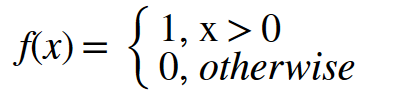
\includegraphics[width=10cm]{img/relu3.png}
      \caption{A derivada da função ReLU} \label{relu3}
   \end{center}
\end{figure}


\subsection[Criando nosso modelo]{Criando nosso modelo}

\begin{lstlisting}[language=Python, caption=Modelo]

class NeuralNet(nn.Module):
    def __init__(self, input_size, hidden_size, num_classes):
        super(NeuralNet, self).__init__()
        self.l1 = nn.Linear(input_size, hidden_size)
        self.l2 = nn.Linear(hidden_size, hidden_size)
        self.l3 = nn.Linear(hidden_size, num_classes)
        self.relu = nn.ReLU()

    def forward(self, x):
        out = self.l1(x)
        out = self.relu(out)
        out = self.l2(out)
        out = self.relu(out)
        out = self.l3(out)
        # sem ativacao e sem softmax no final
        return out

\end{lstlisting}

Aqui nós herdamos uma classe do NN.Module porque estaremos customizando o modelo e suas camadas.


\section[Atribuindo o conjunto de dados ao modelo]{Atribuindo o conjunto de dados ao modelo}

Usaremos algumas funções de Magic, escreva nossa classe.

\textit{Define: funções de Magic} ou Métodos mágicos são métodos especiais em python que possuem sublinhados duplos (dunder) em ambos os lados do nome do método. Métodos mágicos são predominantemente usados para sobrecarga do operador. Sobrecarga de operador significa fornecer funcionalidade adicional aos operadores, o python invoca implicitamente os métodos mágicos para fornecer funcionalidade adicional a ele. Por exemplo, a multiplicação de dois inteiros pode ser feita usando o operador de multiplicação (2*3 = 6) e o mesmo operador pode ser usado para repetir a string (“maçã-” * 3 = ‘maçã- maçã- maçã’).
Alguns exemplos de métodos mágicos são init, len, repr, add e etc \footnote{\url{https://www.analyticsvidhya.com/blog/2021/08/explore-the-magic-methods-in-python}}\footnote{\url{https://www.geeksforgeeks.org/dunder-magic-methods-python/}}.


\begin{itemize}
   \item O método init para inicialização é invocado sem qualquer chamada, quando uma instância de uma classe é criada, como construtores em algumas outras linguagens de programação, como C++, Java, PHP etc. Esses métodos são a razão pela qual podemos adicionar duas strings com ' +' operador sem qualquer typecast explícito.
   \item O método getitem é usado para obter um item do atributo das instâncias invocadas. getitem é comumente usado com contêineres como lista, tupla, etc.
   \item O método mágico len é usado para encontrar o comprimento dos atributos da instância. Quando usamos len(instance), ele retorna o comprimento do atributo de instância que geralmente é um container.
\end{itemize}

\begin{lstlisting}[language=Python, caption=Dataset]
class ChatDataset(Dataset):

    def __init__(self):
        self.n_samples = len(X_train)
        self.x_data = X_train
        self.y_data = y_train

    # suporte a indexacao de modo que o conjunto de dados[i] possa ser usado para obter a i-esima amostra

    def __getitem__(self, index):
        return self.x_data[index], self.y_data[index]

    # podemos chamar len(dataset) para retornar o tamanho
    def __len__(self):
        return self.n_samples

\end{lstlisting}


\section[Hiperparâmetros]{Hiperparâmetros}
Toda rede neural tem um conjunto de hiperparâmetros que precisam ser definidos antes do uso.

Antes de instanciar nossa classe ou modelo de rede neural que escrevemos anteriormente, primeiro definiremos alguns hiperparâmetros que podem ser alterados de acordo.

Os hiperparâmetros são parâmetros cujos valores controlam o processo de aprendizado e determinam os valores dos parâmetros do modelo que um algoritmo de aprendizado acaba aprendendo. O prefixo hyper sugere que são parâmetros de nível superior que controlam o processo de aprendizagem e os parâmetros do modelo que dele resultam.

Um engenheiro de aprendizado de máquina projetando um modelo, faz a escolha de definer valores de hiperparâmetros que seu algoritmo de aprendizado usará antes mesmo do início do treinamento do modelo. Sob essa luz, os hiperparâmetros são considerados externos ao modelo porque o modelo não pode alterar seus valores durante o aprendizado/treinamento\footnote{\url{https://towardsdatascience.com/parameters-and-hyperparameters-aa609601a9ac}}\footnote{\url{https://machinelearningmastery.com/difference-between-a-batch-and-an-epoch}}\footnote{\url{https://www.javatpoint.com/hyperparameters-in-machine-learning}}.


Hiperparâmetros:


\begin{itemize}
   \item  \textit{Define: Epoch} O número de épocas é um hiperparâmetro que define o número de vezes que o algoritmo de aprendizado funcionará em todo o conjunto de dados de treinamento.

         Uma época significa que cada amostra no conjunto de dados de treinamento teve a oportunidade de atualizar os parâmetros internos do modelo.

         Você pode pensar em um loop for sobre o número de épocas em que cada loop prossegue no conjunto de dados de treinamento. Dentro desse loop for há outro loop for aninhado que itera sobre cada lote de amostras, onde um lote tem o número de amostras "tamanho de lote" especificado.

         O número de épocas é tradicionalmente grande, geralmente centenas ou milhares, permitindo que o algoritmo de aprendizado seja executado até que o erro do modelo seja suficientemente minimizado. Você pode ver exemplos do número de épocas na literatura e em tutoriais definidos para 10, 100, 500, 1000 e maiores.

   \item \textit{Define: Batch} O tamanho do Batch é um hiperparâmetro que define o número de amostras para trabalhar antes de atualizar os parâmetros do modelo interno.

         Pense em um Batch como um loop for iterando sobre uma ou mais amostras e fazendo previsões. No final do Batch , as previsões são comparadas com as variáveis de saída esperadas e um erro é calculado. A partir desse erro, o algoritmo de atualização é usado para melhorar o modelo, por exemplo. mover para baixo ao longo do gradiente de erro.

   \item \textit{Define: Learnin Rate} O hiperparâmetro de taxa de aprendizado controla a taxa ou velocidade na qual o modelo aprende. Especificamente, ele controla a quantidade de erro distribuído com o qual os pesos do modelo são atualizados cada vez que são atualizados, como no final de cada lote de exemplos de treinamento.

   \item \textit{Define: Hidden Units} As unidades ocultas fazem parte das redes neurais, que se referem aos componentes que compõem as camadas de processadores entre as unidades de entrada e saída em uma rede neural. É importante especificar o número de hiperparâmetros de unidades ocultas para a rede neural. Deve estar entre o tamanho da camada de entrada e o tamanho da camada de saída. Mais especificamente, o número de unidades ocultas deve ser 2/3 do tamanho da camada de entrada, mais o tamanho da camada de saída.

\end{itemize}


Veja mais sobre Hiperparâmetros aqui\footnote{\url{https://towardsdatascience.com/what-are-hyperparameters-and-how-to-tune-the-hyperparameters-in-a-deep-neural-network-d0604917584a}}.




\begin{lstlisting}[language=Python, caption=Hiperparâmetros]
# Hiperparametros
num_epochs = 1000
batch_size = 8
learning_rate = 0.001
input_size = len(X_train[0])
hidden_size = 8
output_size = len(tags)
print(input_size, output_size)

\end{lstlisting}

\section[Perda e otimizador]{Perda e otimizador}

Vamos agora instanciar as funções de modelo, perda e otimizador.

Função de Perda: Cross Entropy
Otimizador: Adam Optimizer

\begin{lstlisting}[language=Python, caption=Perda e otimizador]
dataset = ChatDataset()
train_loader = DataLoader(dataset=dataset,
                          batch_size=batch_size,
                          shuffle=True,
                          num_workers=0)

device = torch.device('cuda' if torch.cuda.is_available() else 'cpu')

model = NeuralNet(input_size, hidden_size, output_size).to(device)

# Perda e otimizador
criterion = nn.CrossEntropyLoss()
optimizer = torch.optim.Adam(model.parameters(), lr=learning_rate)

\end{lstlisting}

\section[Treinando o Modelo]{Treinando o Modelo}

\begin{lstlisting}[language=Python, caption=Treinando o Modelo]

# Treine o modelo
for epoch in range(num_epochs):
    for (words, labels) in train_loader:
        words = words.to(device)
        labels = labels.to(dtype=torch.long).to(device)

        # Forward pass
        outputs = model(words)
        # if y would be one-hot, we must apply
        # labels = torch.max(labels, 1)[1]
        loss = criterion(outputs, labels)

        # Backward e optimize
        optimizer.zero_grad()
        loss.backward()
        optimizer.step()

    if (epoch+1) % 100 == 0:
        print (f'Epoch [{epoch+1}/{num_epochs}], Loss: {loss.item():.4f}')


print(f'final loss: {loss.item():.4f}')

data = {
"model_state": model.state_dict(),
"input_size": input_size,
"hidden_size": hidden_size,
"output_size": output_size,
"all_words": all_words,
"tags": tags
}


\end{lstlisting}

\begin{figure}[H]
   \begin{center}
      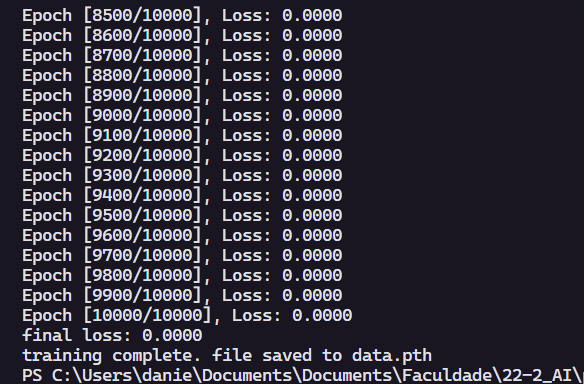
\includegraphics[width=10cm]{img/treinando.png}
      \caption{output} \label{tmode}
   \end{center}
\end{figure}


\subsection[Salvando o modelo treinado]{Salvando o modelo treinado}

\begin{lstlisting}[language=Python, caption=Salvando o modelo treinado]

FILE = "data.pth"
torch.save(data, FILE)

print(f'training complete. file saved to {FILE}')

\end{lstlisting}

section[Carregando nosso modelo salvo]{Carregando modelo salvo}

\begin{lstlisting}[language=Python, caption=Carregando modelo salvo]

device = torch.device('cuda' if torch.cuda.is_available() else 'cpu')

with open('intents.json', 'r') as json_data:
    intents = json.load(json_data)

FILE = "data.pth"
data = torch.load(FILE)

input_size = data["input_size"]
hidden_size = data["hidden_size"]
output_size = data["output_size"]
all_words = data['all_words']
tags = data['tags']
model_state = data["model_state"]

model = NeuralNet(input_size, hidden_size, output_size).to(device)
model.load_state_dict(model_state)
model.eval()

\end{lstlisting}

\section[Usando o Chatbot]{Usando o Chatbot}

Nosso modelo está pronto. Agora vamos finalmente conversar com nosso chatbot. Como nossos dados de treinamento eram muito limitados, só podemos conversar sobre alguns tópicos. O modelo pode ser treinado em um conjunto de dados maior para aumentar a generalização/conhecimento do Chatbot.

\begin{lstlisting}[language=Python, caption=Chatbot]

bot_name = "chatbotIA"
print("Let's chat! (digite 'quit' para sair)")
while True:
    # frase = "Ola!"
    sentence = input("Voce: ")
    if sentence == "quit":
        break

    sentence = tokenize(sentence)
    X = bag_of_words(sentence, all_words)
    X = X.reshape(1, X.shape[0])
    X = torch.from_numpy(X).to(device)

    output = model(X)
    _, predicted = torch.max(output, dim=1)

    tag = tags[predicted.item()]

    probs = torch.softmax(output, dim=1)
    prob = probs[0][predicted.item()]
    if prob.item() > 0.75:
        for intent in intents['intents']:
            if tag == intent["tag"]:
                print(f"{bot_name}: {random.choice(intent['responses'])}")
    else:
        print(f"{bot_name}: Eu nao entendi...")


\end{lstlisting}

Nosso Modelo foi treinado com pouquíssimos exemplos, então não entende tudo o que passamos para ele.

% ---

% ----------------------------------------------------------
% PARTE
% ----------------------------------------------------------
%\part{Referenciais teóricos}
% ----------------------------------------------------------

% ---
% Capitulo de revisão de literatura

% ---



% ----------------------------------------------------------
% PARTE
% ----------------------------------------------------------
%\part{Resultados}
% ----------------------------------------------------------

% ---
% primeiro capitulo de Resultados
% ---

% ---

% ---


% ---
% segundo capitulo de Resultados
% ---


% ----------------------------------------------------------
% Finaliza a parte no bookmark do PDF
% para que se inicie o bookmark na raiz
% e adiciona espaço de parte no Sumário
% ----------------------------------------------------------
\phantompart

% ---
% Conclusão
% ---
%\chapter{Conclusão}
% ---


% ----------------------------------------------------------
% ELEMENTOS PÓS-TEXTUAIS
% ----------------------------------------------------------
\postextual
% ----------------------------------------------------------

% ----------------------------------------------------------
% Referências bibliográficas
% ----------------------------------------------------------
\bibliography{abntex2-modelo-references}

% ----------------------------------------------------------
% Glossário
% ----------------------------------------------------------
%
% Consulte o manual da classe abntex2 para orientações sobre o glossário.
%
%\glossary

% ----------------------------------------------------------
% Apêndices
% ----------------------------------------------------------

% ---
% Inicia os apêndices
\begin{comment}
% ---
\begin{apendicesenv}

	% Imprime uma página indicando o início dos apêndices
	\partapendices



	% ----------------------------------------------------------
	%\chapter{Quisque libero justo}
	% ----------------------------------------------------------

	\lipsum[50]

	% ----------------------------------------------------------
	\chapter{Nullam elementum urna vel imperdiet sodales elit ipsum pharetra ligula
	  ac pretium ante justo a nulla curabitur tristique arcu eu metus}
	% ----------------------------------------------------------
	\lipsum[55-57]

\end{apendicesenv}
% ---


% ----------------------------------------------------------
% Anexos
% ----------------------------------------------------------

% ---
% Inicia os anexos
% ---
\begin{anexosenv}

	% Imprime uma página indicando o início dos anexos
	\partanexos

	% ---
	%\chapter{Morbi ultrices rutrum lorem.}
	% ---
	\lipsum[30]

	% ---
	%\chapter{Cras non urna sed feugiat cum sociis natoque penatibus et magnis dis
	%parturient montes nascetur ridiculus mus}
	% ---

	\lipsum[31]

	% ---
	%\chapter{Fusce facilisis lacinia dui}
	% ---

	\lipsum[32]

\end{anexosenv}

\end{comment}
%---------------------------------------------------------------------
% INDICE REMISSIVO
%---------------------------------------------------------------------
\phantompart
\printindex
%---------------------------------------------------------------------

\end{document}
